\saltoPag{}
\section{UNIDAD 4}
    \begin{center}
        \begin{tabular}{| m{2.25cm} | m{2.25cm} | m{2.25cm} |}
            \hline
            \multicolumn{3}{| c |}{\textcolor{red}{\textbf{ESTADOS DE AGREGACIÓN}}} \\
            \hline
            \multirow{1}{2.25cm}{\centering\textbf{Sólidos}} &
            \multirow{1}{2.25cm}{\centering\textbf{Líquidos}} &
            \multirow{1}{2.25cm}{\centering\textbf{Gases}} \\
            \hline
            Forma definida & Volumen definido & Forma y volumen del recipiente que lo contiene. \\
            \hline
            Volumen definido & Forma del recipiente que lo contiene & Muy compresible \\
            \hline
            No comprensibles & No comprensibles & Movimiento muy libre \\
            \hline
            Partículas ordenadas con movimiento de vibración & Las partículas se deslizan entre sí libremente & \\
            \hline
        \end{tabular}
    \end{center}
    \begin{center} 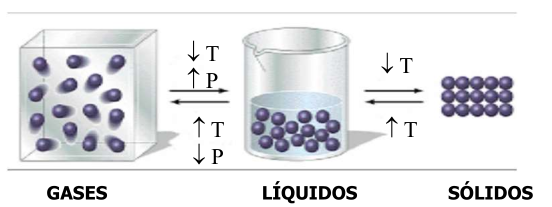
\includegraphics[width=7cm]{./imagenes/estadosDeAgregacionMoleculas.png} \end{center}
    \subsection{Líquidos}
        \subsubsection{Viscosidad}
            \sangria{} Medida de la resistencia de un líquido para fluir.
            \begin{center} 
                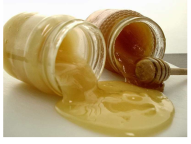
\includegraphics[width=4cm]{./imagenes/miel.png} \\[15pt]
                \textit{El aumento de la temperatura implica menor viscosidad.}
            \end{center}
            \begin{center} 
                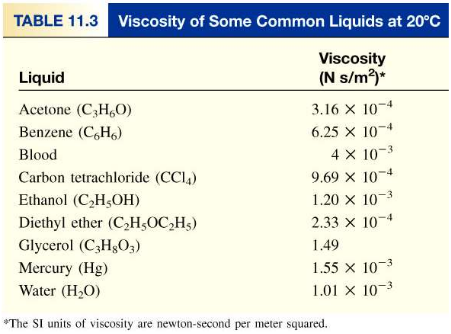
\includegraphics[width=6cm]{./imagenes/tablaViscosidad.png} \\[15pt]
                \textit{Las fuerzas inter-moleculares fuertes implican una alta viscosidad.}
            \end{center}

        \subsubsection{Tensión superficial}
            \sangria{} Cantidad de energía requerida para dilatar o aumentar la superficie de un líquido por unidad de área.
            \begin{center} 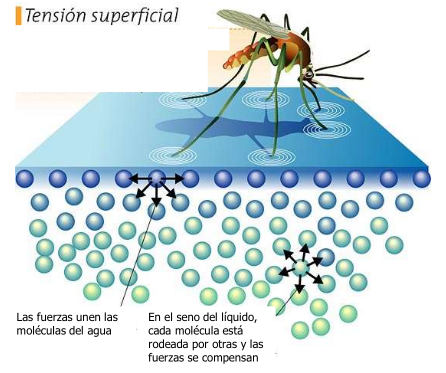
\includegraphics[width=6cm]{./imagenes/mosquitoTensionSuperficial.png} \end{center}
            \begin{center} \textcolor{red}{\underline{Capilaridad:} ejemplo de tensión superficial} \end{center}
            \sangria{} Es el resultado de dos fuerzas:
            \begin{itemize}
                \item \textbf{Cohesión:} atracción inter-molecular entre moléculas similares.
                \item \textbf{Adhesión:} atracción inter-molecular entre moléculas diferentes.
            \end{itemize}
            \begin{center} 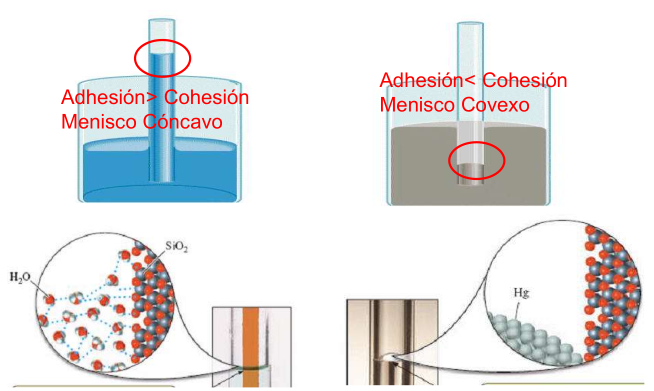
\includegraphics[width=6cm]{./imagenes/fuerzasCapilaridad.png} \end{center}
            \begin{center} 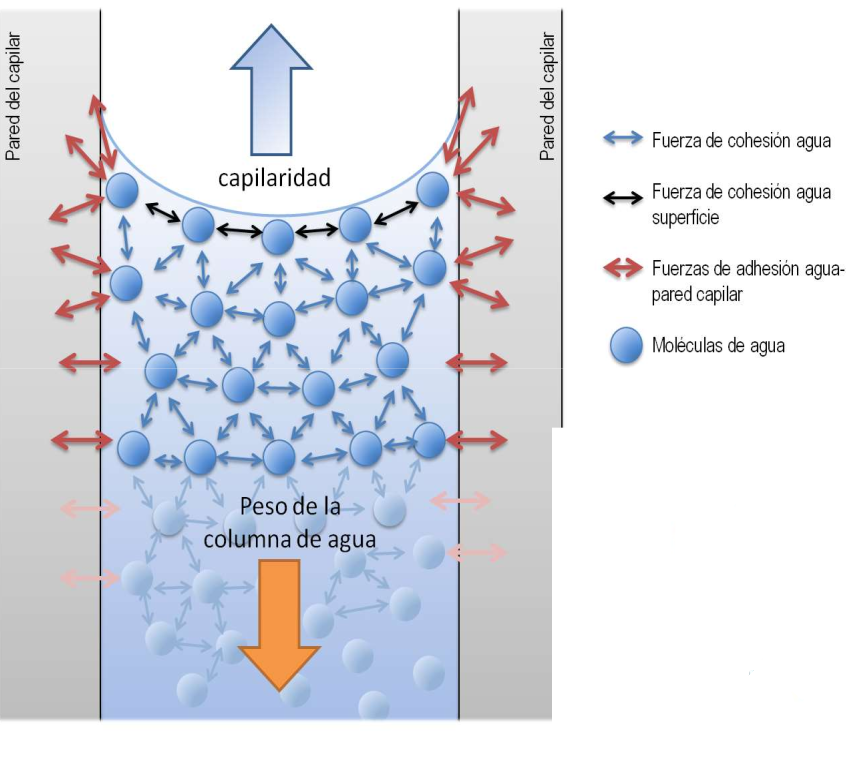
\includegraphics[width=8cm]{./imagenes/detallesCapilaridad1.png} \end{center}
            \begin{center} 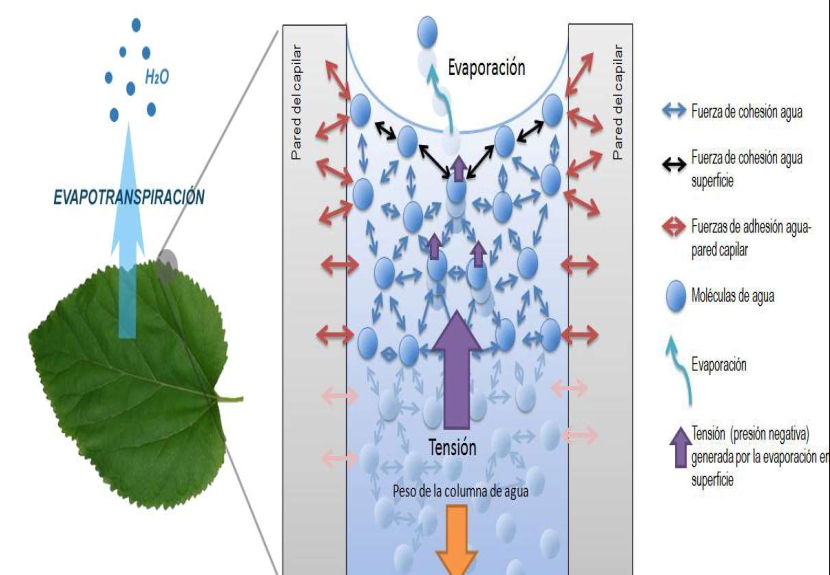
\includegraphics[width=8cm]{./imagenes/detallesCapilaridad2.png} \end{center}
        \saltoPag{}
        \subsubsection{Evaporación y presión de vapor}
            \sangria{} \underline{Conceptos:}
            \begin{itemize}
                \item \textbf{Presión de vapor:} presión ejercida por el vapor de un líquido sobre la superficie del mismo cuando el líquido y el vapor se encuentran en equilibrio dinámico a una temperatura determinada.
            \end{itemize}
            \begin{center} 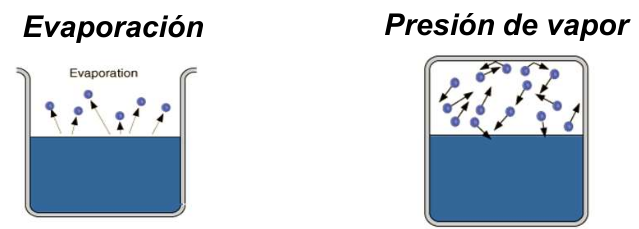
\includegraphics[width=5cm]{./imagenes/evaporacionYPresionDeVapor.png} \end{center}
            \begin{center}
                \begin{tabular}{ | m{1.8cm} | m{1cm} | m{1cm} | m{1cm} | m{1.3cm} |}
                    \hline
                    \multicolumn{5}{| c |}{\textcolor{red}{\textbf{Presión de vapor (Torr)}}} \\
                    \hline
                    \textbf{Compuesto} & \centering $\ang{0}C$ & \centering $\ang{20}C$ & \centering $\ang{30}C$ & \scriptsize \textbf{Punto de ebullición normal ($1atm$)} \\
                    \hline
                    Dietileter & 185 & 442 & 647 & $\ang{36}C$ \\
                    \hline
                    Etanol & 12 & 44 & 74 & $\ang{78}C$ \\
                    \hline
                    Agua & 5 & 18 & 32 & $\ang{100}C$ \\
                    \hline
                \end{tabular}
            \end{center}
            \begin{itemize}
                \item \textbf{Punto de ebullición:} es la temperatura en la cual la presión de vapor (en equilibrio) de un líquido es igual a la presión externa.
                \item \textbf{Punto de ebullición normal:} es la temperatura en la cual un líquido hierve cuando la presión externa es de $1atm$.
            \end{itemize}
            \begin{center} 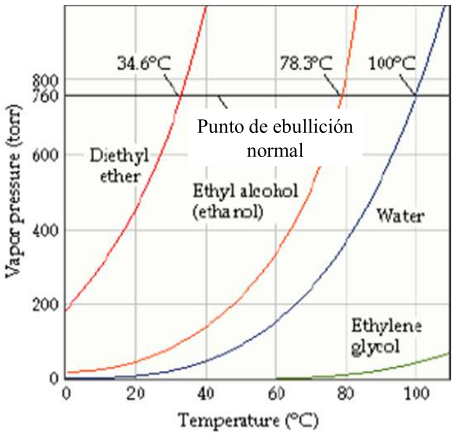
\includegraphics[width=7cm]{./imagenes/puntoDeEbullicion.png} \end{center}
            \begin{itemize}
                \item \textbf{Temperatura crítica ($T_C$):} temperatura por arriba de la cual el gas no puede licuarse, no importa cuán grande sea la presión aplicada.
                \item \textbf{Presión crítica ($P_C$):} es la presión mínima que debe aplicarse para ocasionar licuefacción a la temperatura crítica.
            \end{itemize}
            \begin{center} 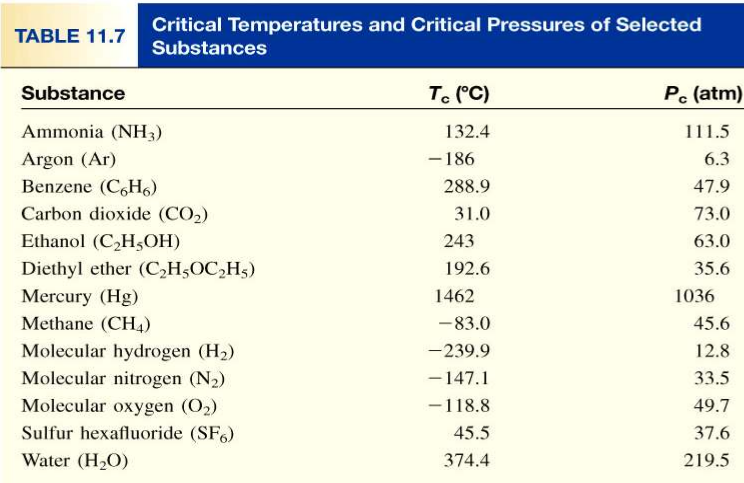
\includegraphics[width=8cm]{./imagenes/presionYTemperaturaCritica.png} \end{center}
            \begin{itemize}
                \item \textbf{Diagrama de fases:} resume las condiciones en las cuales una sustancia existe como sólido, líquido o gas.
            \end{itemize}
            \begin{center} 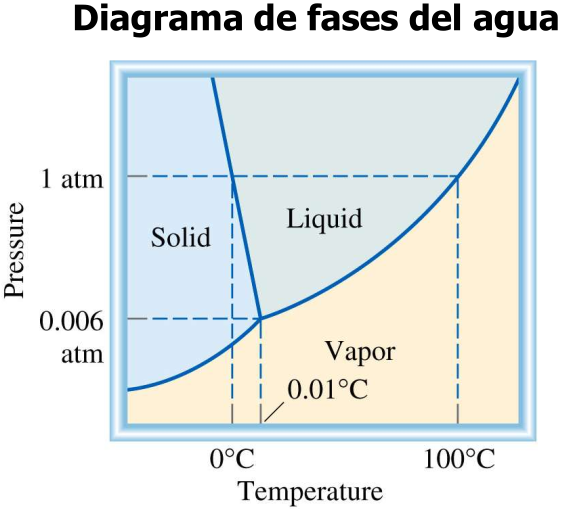
\includegraphics[width=6cm]{./imagenes/diagramaDeFasesDelAgua.png} \end{center}
            \begin{center} 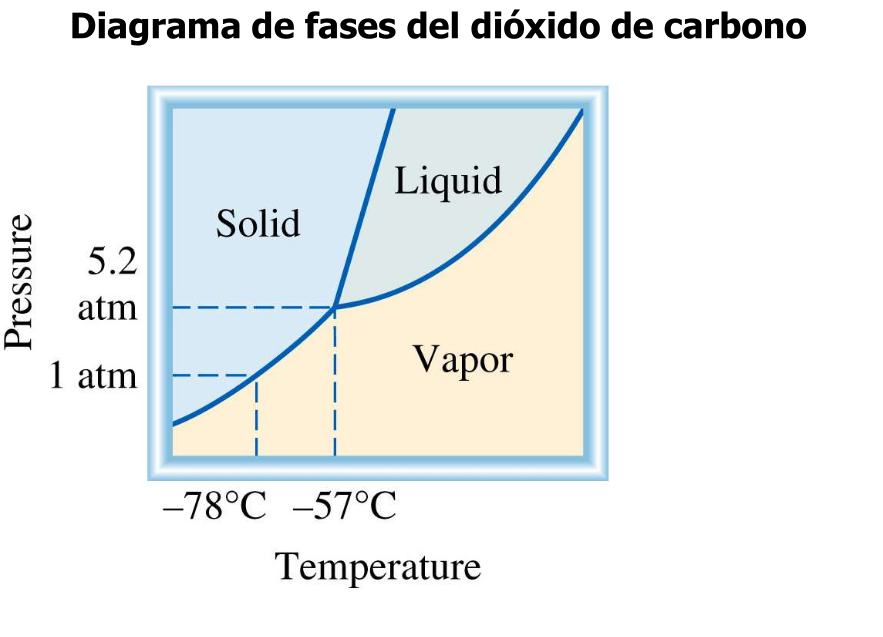
\includegraphics[width=6cm]{./imagenes/diagramaDeFasesDelCO2.png} \end{center}
    \subsection{Gases}
        \sangria{} Los siguientes elementos pueden existir como gases a una temperatura de $\ang{25}C$ y a $1atm$ de presión.
        \begin{center} 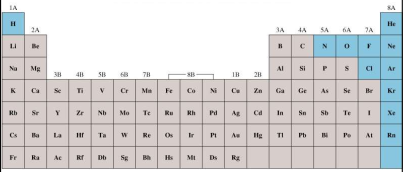
\includegraphics[width=7cm]{./imagenes/elementosGasACondNormales.png} \end{center}
        \saltoPag{}
        \begin{center} 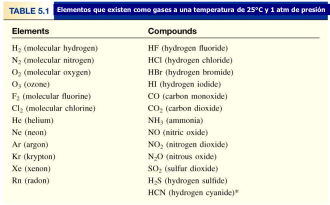
\includegraphics[width=7cm]{./imagenes/elementosGasACondNormales1.png} \end{center}
        \subsubsection{Características físicas de los gases}
        \begin{itemize}
            \item Son capaces de adquirir cualquier forma.
            \item Compresibles.
            \item Pueden mezclarse con todo tipo de elementos con mucha facilidad.
            \item Tienen una densidad mucho menor que los sólidos y los líquidos.
        \end{itemize}
        \subsubsection{Presión atmosférica}
            \sangria{} Se recuerda que:
            \begin{center} 
                $ P_{\text{PRESIÓN}} = \frac{F_{FUERZA}}{A_{\text{ÁREA}}} $
            \end{center}
            \begin{center}
                \begin{tabular}{| m{3.5cm} | m{3.5cm} |}
                    \hline
                    \multicolumn{2}{| c |}{\textcolor{blue}{\textbf{Unidades de presión}}} \\
                    \hline
                    $1Pa$ (Pascal) & 1 N/$m^2$ \\
                    \hline
                    $1atm$ (Atmósfera) & $760 mmHg$ (mm mercurio) \\
                    \hline
                    $1mmHg$ & $1 Torr$ \\
                    \hline
                    $1atm$ & $101,325 Pa$ \\
                    \hline
                \end{tabular}
            \end{center}
            \begin{center} 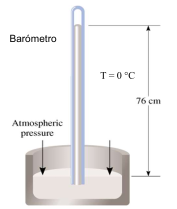
\includegraphics[width=3cm]{./imagenes/barometro.png} \end{center}
